\chapter{Data Bills}
\label{cha:data-bills}

\section{95th Percentile}
\label{sec:95th-percentile}

\textit{95th percentile} is a commonly used commercial scheme to
calculate and evaluate the regular and sustained used of a network
connection. It is a kind of
\href{https://en.wikipedia.org/wiki/Burstable_billing}{Burstable
  Billing} that measures bandwidth based on \textit{peak use}.

Generally, it allows the usage to exceed a specified threshold for
a short period of time without the financial penalty of purchasing
a higher
\href{https://en.wikipedia.org/wiki/Committed_information_rate}{Committed
  Information Rate} (CIR is another billing method) from an ISP.

There are two critical factors involved in this scheme, namely the
\textit{percentile} and the \textit{sampling interval}. Usually,
they are 95 and 5 respectively and therefore it is also called
\textit{95/5 percentile.}

Given a monthly billing cycle, 95/5 percentile allows a customer
to have a short (i.e. threshold is $30 \times 24 \times 5\% = 36$
hours) burst in in traffic without overage charges. That is to
say, 95\% of the time, the usage is below this
ammount. Conversely, 5\% of the samplings may be bursting above
this rate.

\begin{figure}[!htbp]
  \centering
  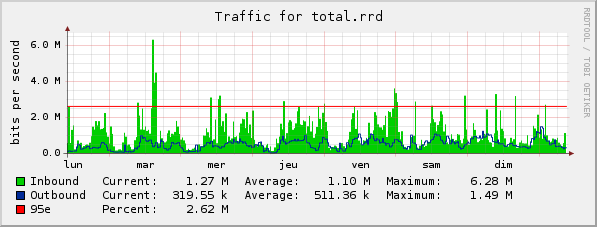
\includegraphics[scale=.6]{burstableBilling}
  \caption{95/5 Percentile}
  \label{fig:95-percentile}
\end{figure}

How is \textit{this ammount} or \textit{this rate} is calculated?
Usually a time-bandwidth chart is drawn to visualize bandwidth
usage through a bill cyle like figure \ref{fig:95-percentile}
whose \textit{integral area} reflects the total data transmitted.

Bandwidth is sampled at an interval of 5 minutes from the switch
or router. During an interval, the average bandwidth is calculated
as the number of bits transferred throughout the interval divided
by the duration (5m = 300s).

At the end of the month, all the bandwidth samples
($30 \times 24 \times 60 \div 5 = 8640$) are sorted from highest
to lowest. The top 5\% ($8640 \times 5\% = 432$) samples is thrown
away and the next highest sample \uline{433} becomes the billable
use for the entire month.

Obviously, $432 \times 5 \div 60 = 36$. More specifically,
bandwidth could be used at a higher rate for up to
$24 \times 60 \times 5\% = 72$ minutes a day with no financial
penalty.

In the figure \ref{fig:sorted-95th-percentile}, the
billable value falls around 6Mbps, or 60\% of the highest
burst. From this figure, we find the sorted slope is quite
steep. The sharp burst contributes a lot to the final bill though
not much bandwidth is used.

\begin{figure}[!htbp]
  \centering
  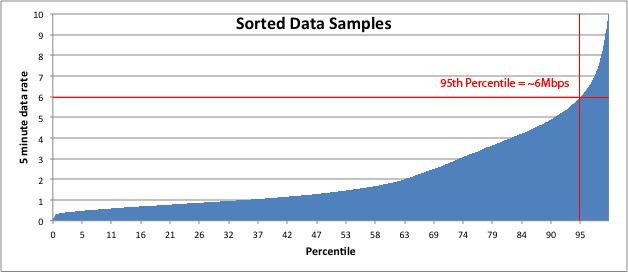
\includegraphics[scale=.5]{95th-chart-sorted}
  \caption{Sorted Percentile}
  \label{fig:sorted-95th-percentile}
\end{figure}

Conversely, at any moment during the billing cycle, even if peak
traffic only appears for a short \textit{instant} and no
additional traffic is generated, the billing ammount can be
sbustantially higher than average usage billing.

This is not the end of the story. Although we get the billable
value, it may not take affect when paying bills. For example, what
if all customers' 95th percentile valie are pretty small? In that
case, the ISP's infrastructure would be wasted and lose money.

95th percentile also assumes a \textit{base commit rate} (and fees
associated) that must be guranteed by customers. If the 95th
percentile value only take effect when it is higher than the base
commit rate, otherwise the later value is used irrespective of the
real 95th percentile value. The higher the base commit rate is,
the cheaper the bandwidth fee becomes.

Base commit rate is \textit{not} CIR where bandwidth must be
reserved for a customer but just a billing gurantee even the real
bandwidth usage is 0.

Base commit rate is fairly to both the carrier and the customer in
terms of the service delivered to the customer and the ability of
the carrier to scale its infrastructure to meed different
customers' needs.

\section{Other Billing Methods}
\label{sec:other-billing-methods}

The 95th percentile is utilized mostly between ISP and business
customers in a datacenter while CIR is adopted between ISP and
individuals for home cable, fiber, DSL etc. Hard bandwidth is
guranteed and no burst is allowed. Customers pay for the fixed
bandwidth value.

Apart from 95th percentile and CIR, \textit{actual throughput
  billing} is used in limited and shared bandwidth networks like
mobile data networks (i.e. 4G) where where resources
overprovisioning is not possible due to limited spectrum
availability. Customers just pay for what they get on demand. ISP
will simply record how much data you moved over the circuit for
that interval. It is also used by some web-based VPS platforms to
bill customers.

You may think of \textit{average rage bill} where customers pay
for their average committed bandwidth. However, this scheme
requires infrastructure overprovisioning on the part of ISP to
meet customers' peak bandwidth usage. It is not used in real
world!

You can read more about billing methods on
\href{https://www.semaphore.com/95th-percentile-bandwidth-metering-explained-and-analyzed/}{billing
  methods explained and analyzed}.

%%% Local Variables:
%%% mode: latex
%%% TeX-master: "main"
%%% End:
